
\subsection{Characteristics of the network}

The network we used consists of 384 nodes. The distribution of the number of friends and the local clustering coefficients are shown in Figure \ref{hist1}. The one of the betweenness centrality in Figure \ref{hist2}.


\begin{minipage}{0.5\textwidth}
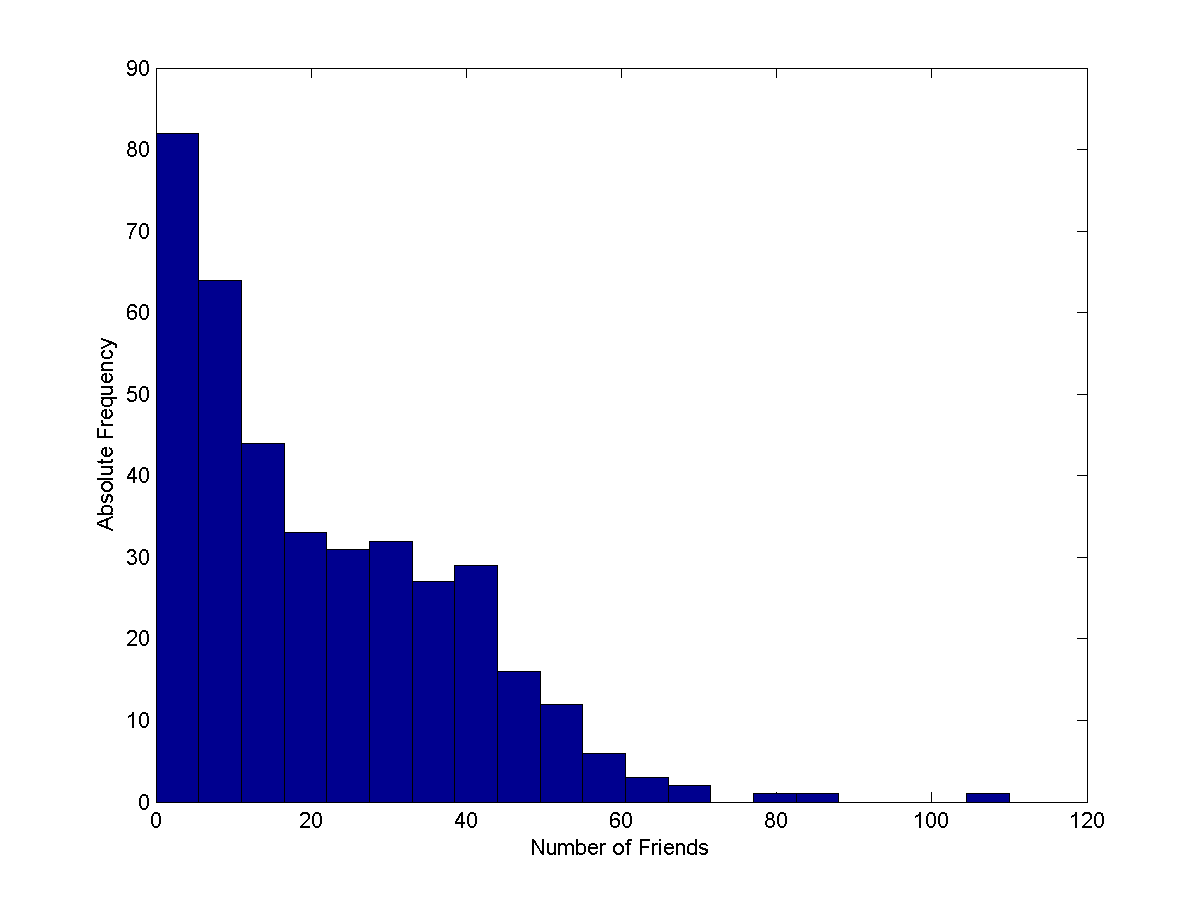
\includegraphics[width=7cm]{network_degreehist.png}
\end{minipage}
\begin{minipage}{0.5\textwidth}
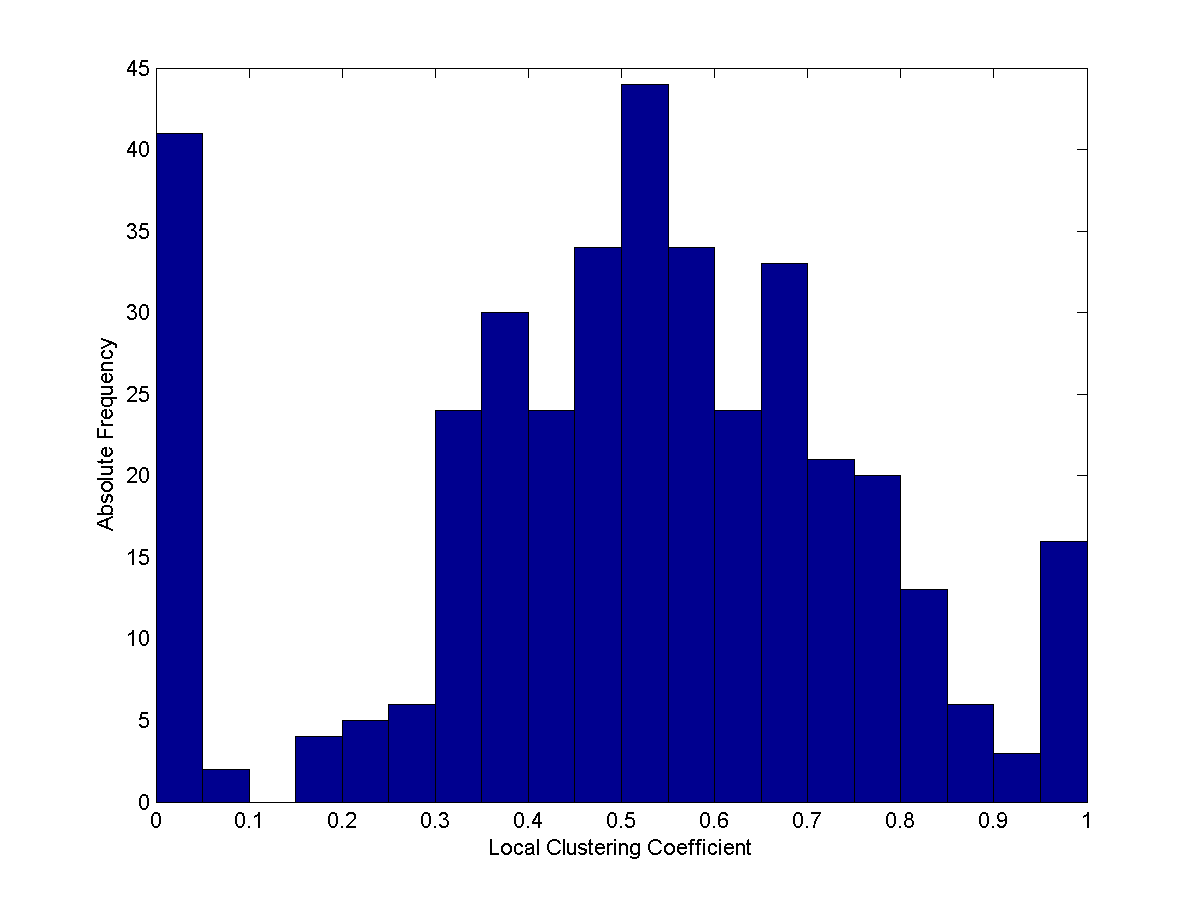
\includegraphics[width=7cm]{network_clusterhist.png}
\end{minipage}
\captionof{figure}{Distribution of the number of friends (left) and the local clustering coefficient (right).}
\label{hist1}


\begin{minipage}{0.5\textwidth}
The main problem of our network is, that it consists of all the friends of one of the authors, with the author removed. The probability of infecting another person was dependent on the mutual friends, so it's possible that two individuals have a lot of common friends in reality, but it appears that they don't because the author doesnn't know these common friends.
\end{minipage}
\begin{minipage}{0.5\textwidth}
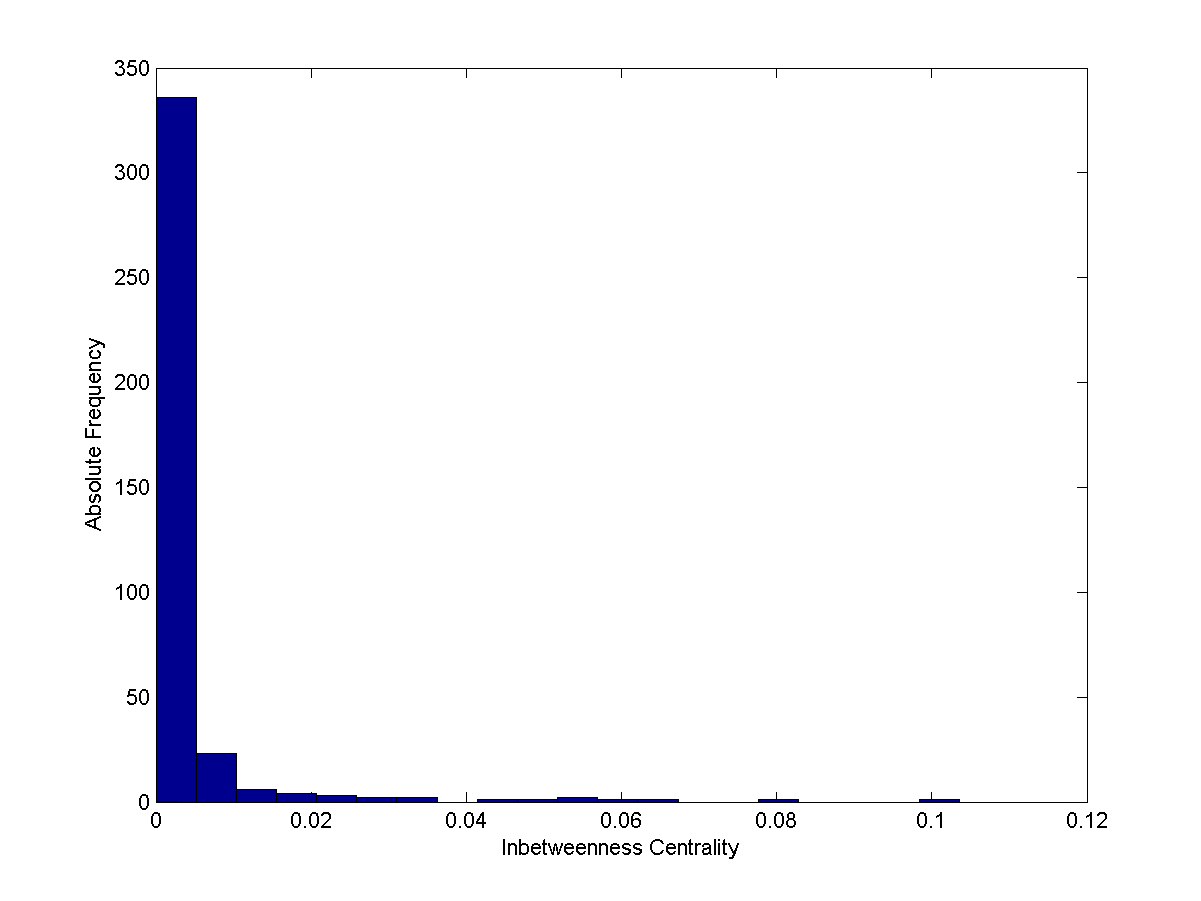
\includegraphics[width=7cm]{network_centralityhist.png}
\captionof{figure}{Distribution of betweenness centrality.}
\label{hist2}
\end{minipage}

%\begin{minipage}{0.33\textwidth}
%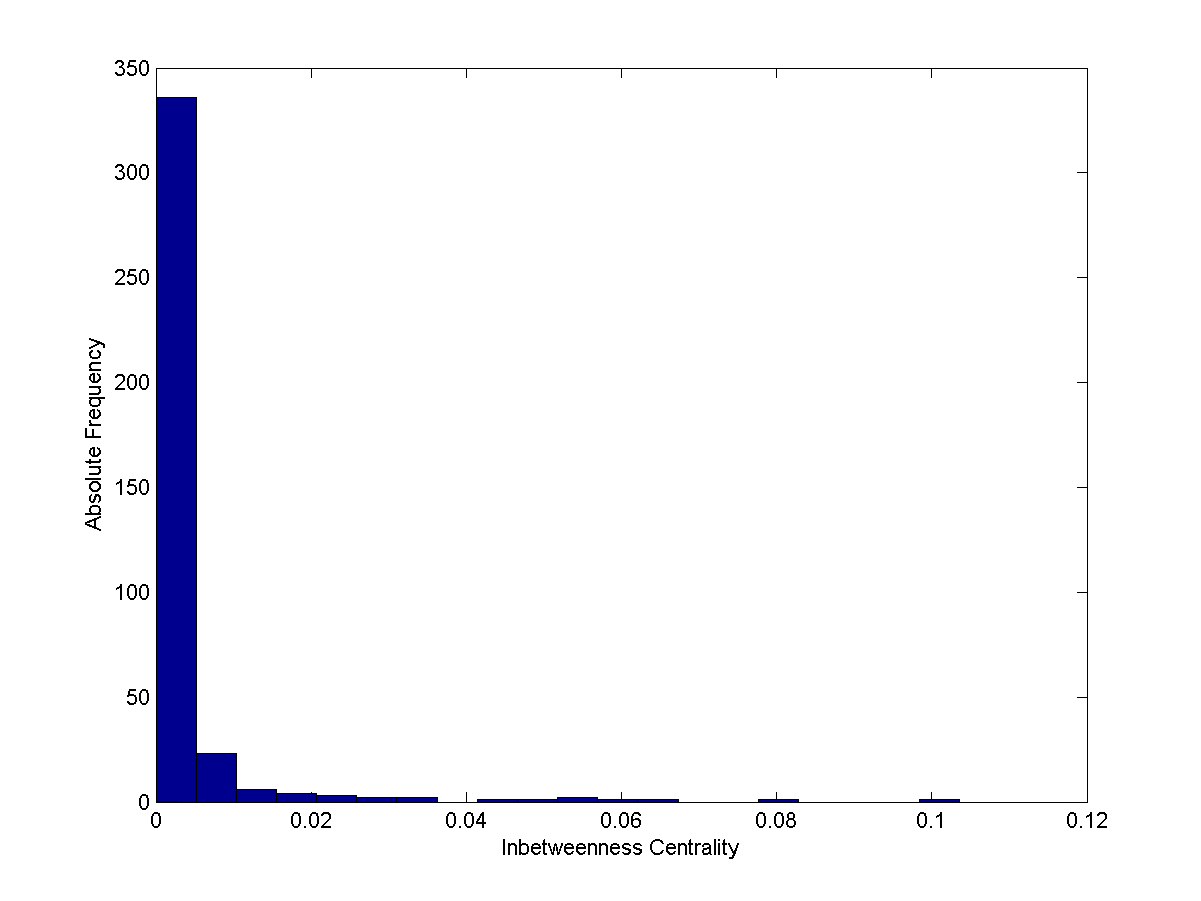
\includegraphics[scale=0.3]{network_centralityhist.png}
%\end{minipage}



\subsection{Differences in the time evolution}

Most of the time, the form of the evolution graph of the system looks very similar in the case of the homogeneous and the inhomogeneous, agent-based model (Figure \ref{evolution1}).

\begin{minipage}{0.5\textwidth}
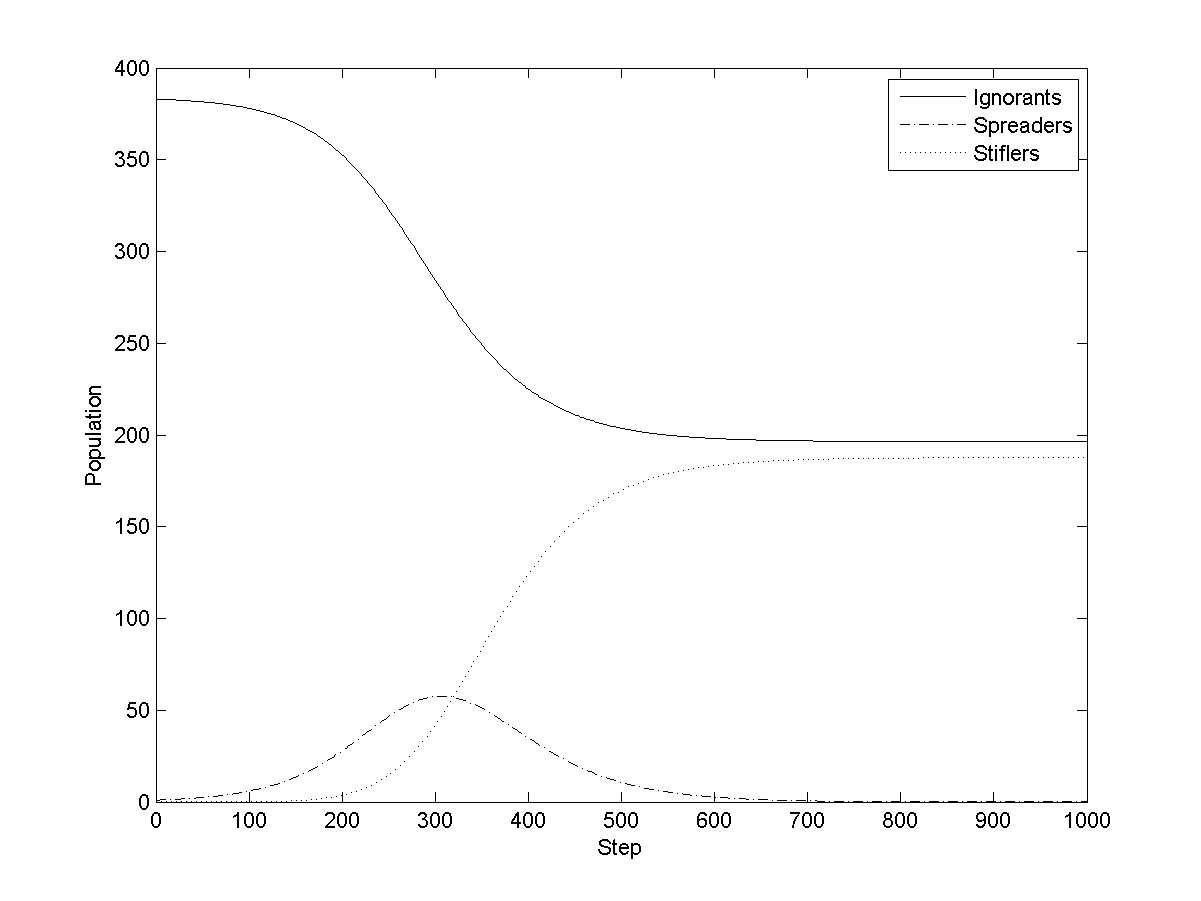
\includegraphics[width=7cm]{NICE_SIR}
\end{minipage}
\begin{minipage}{0.5\textwidth}
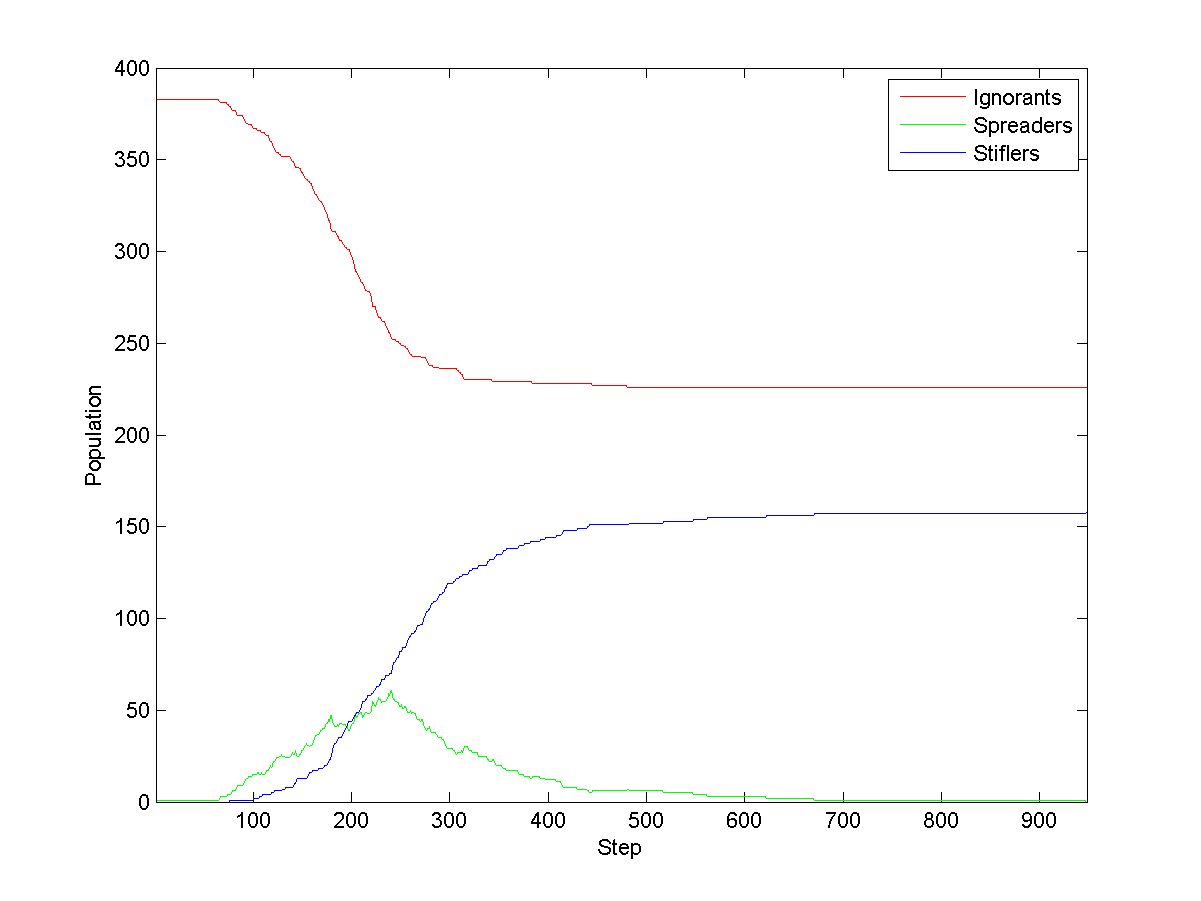
\includegraphics[width=7cm]{1-local-max}
\end{minipage}
\captionof{figure}{Left: Typical evolution of the system in the homogeneous SIR-model. Right: The Evolution in the agent-based model. In most cases, the evolution looks somewhat like this.\newline}
\label{evolution1}


\begin{minipage}{0.5\textwidth}
But there were also interesting cases where two local maxima occurred, as in Figure \ref{2peaks}. This can never be the case in a homogeneous model. This requires several neighbourhoods in the network (and some luck, since the simulation uses random numbers). This might be a rather obvious insight, but it proofs that a homogeneous model might fail totally. If you would base any decision on a homogeneous model and you recognize that the number of spreaders decreases, you would expect that the spreading comes to an end. But it might be  that it hardly started if you have inhomogeneities.
\end{minipage}
\begin{minipage}{0.5\textwidth}
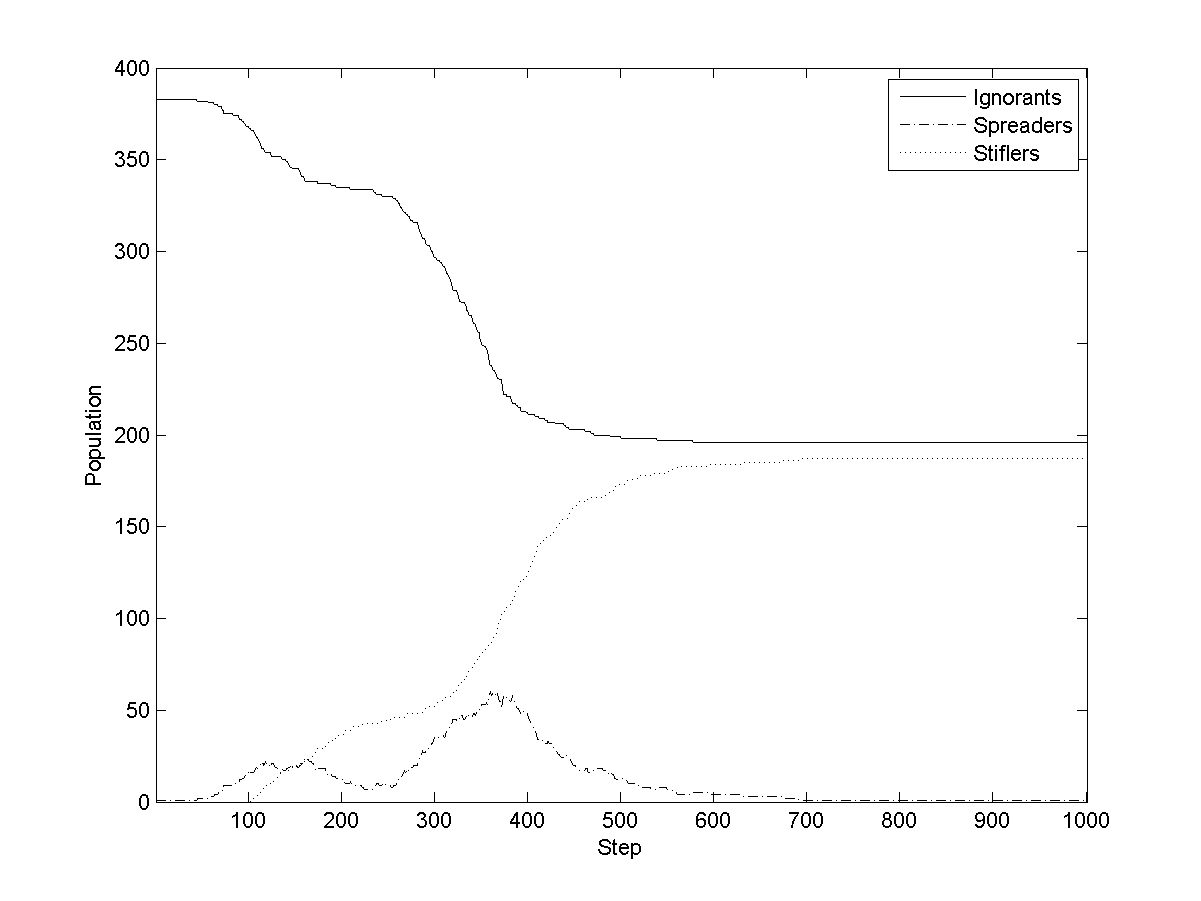
\includegraphics[width=7cm]{2-local-max}
\captionof{figure}{two local maxima, not continuous}
\label{2peaks}
\end{minipage}




\subsection{Influence of $\alpha$}
As shown if figures \ref{SIR_ODE} and \ref{Analysis_pforget} the number of ignorants at the end of the simulation increases for higher $\alpha$ ($\lambda$ is kept constant).

SIR: max of spreaders and the number of ignorants at the end are lower for lower pfoerget (lamda always the same).

\begin{figure}[H!]
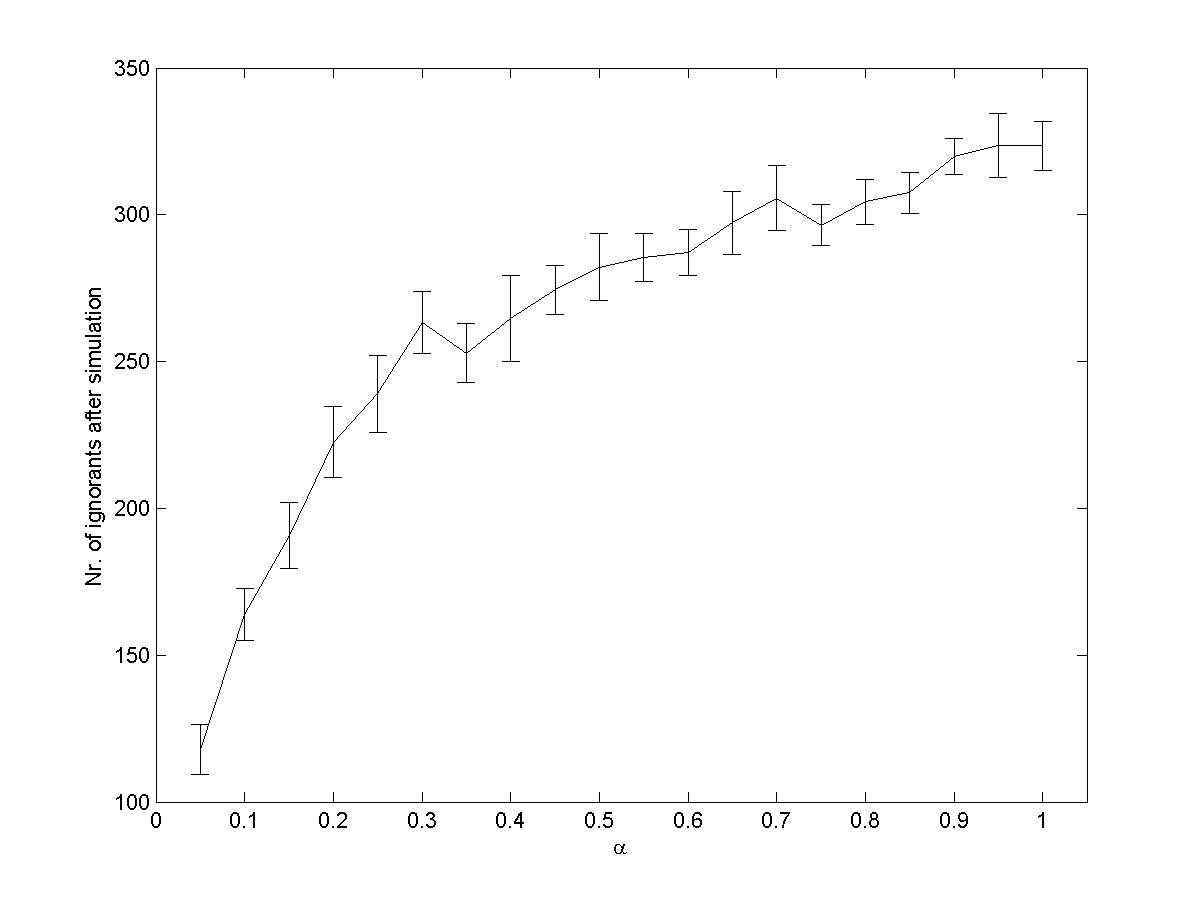
\includegraphics[width=7cm]{Analysis_pforget}
\caption{sdlhfa}
\label{Analysis_pforget}
\end{figure}

\begin{figure}[H!]
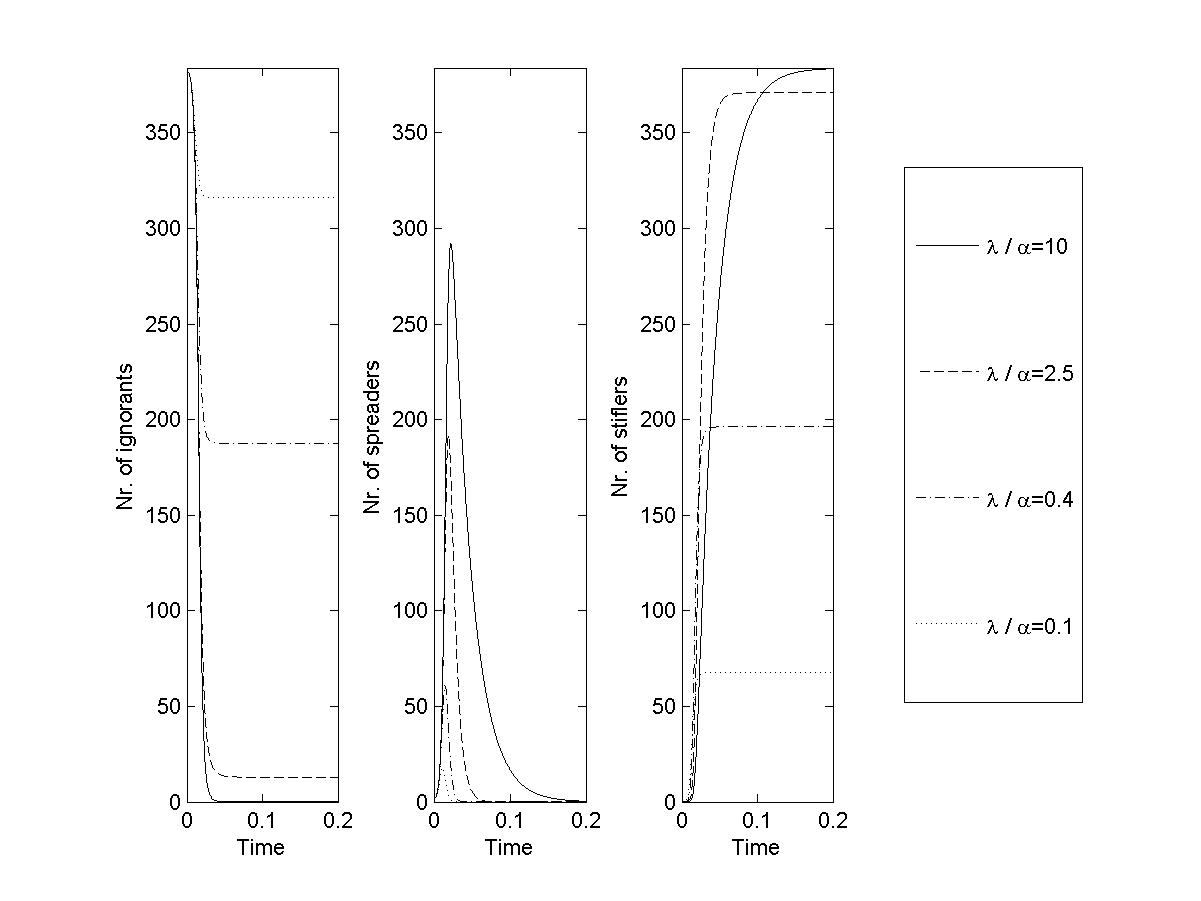
\includegraphics[width=14cm]{SIR_ODE}
\caption{sdlhfa}
\label{SIR_ODE}
\end{figure}
\clearpage
\subsection{Influentials}


\subsubsection{Existance and importance of influentials}


\begin{minipage}{0.5\textwidth}
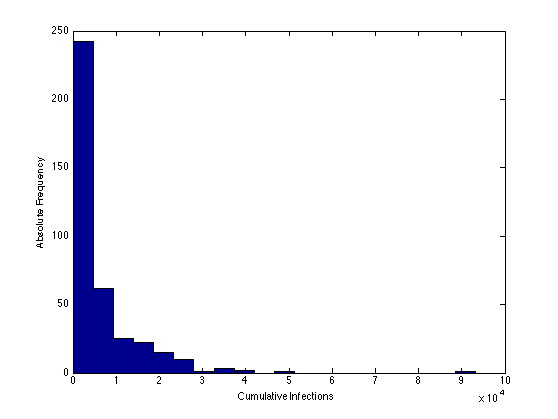
\includegraphics[width=7cm]{influ2}
\caption{Distribution of the cumulative infections, summed over all 3840 rounds. \newline}
\label{Histo}
\end{minipage}
\begin{minipage}{0.5\textwidth}
Figure \ref{Histo} is a simple histogram, that shows that the vast majority of people has only a small cumulative infection value. However, there are some individuals with a very high value. This an indicator for the existence of influentials.   \\
\end{minipage}

%\begin{figure}[H!]
%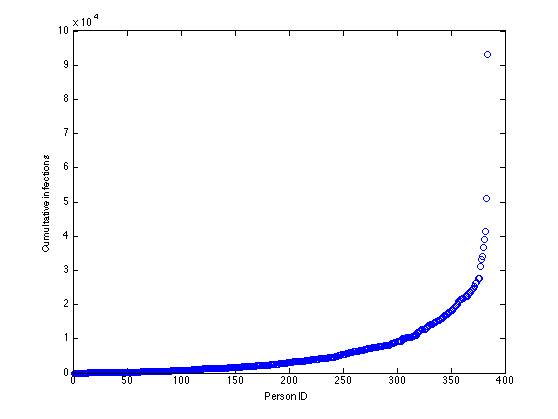
\includegraphics[width=7cm]{influ1}
%\caption{sdlhfa}
%\label{Sorted}
%\end{figure}



\noindent One can even go one step further and try to estimate the importance of those influentials on all infections that occurred in total. In order to do so, the persons are sorted according to their value of cumulative infections. Then, for each person m, we sum up all the infections that occurred in rounds where m itself did NOT infect anybody. Let's call this function f(m). Figure \ref{importancedist} shows the value of $$g(m)=\sum_{i=1}^m f(i) $$
This can be interpreted as the number of infections that occurred in rounds where all persons more or equally important than m did NOT infect anybody. So $g(1)=0$ and $g_{max}=$total infections.
\\
Given these results, we get that 94\% of all infections happen in the rounds where the 1\%-quantile of the most important people were not excluded. 


\begin{minipage}{0.5\textwidth}
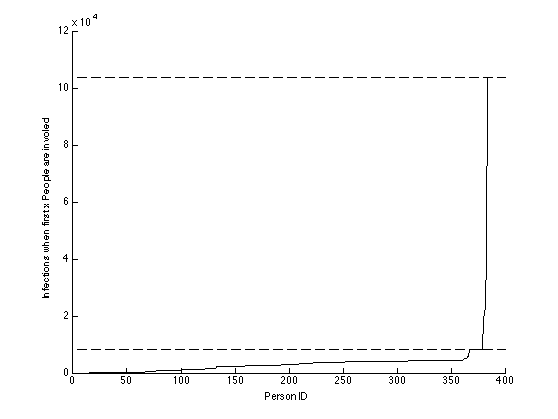
\includegraphics[width=7cm]{influ3}
\end{minipage}
\begin{minipage}{0.5\textwidth}
\caption{ g(m) (see above for details). The bottom dashed line indicated the number of all infections in rounds where the four most important individuals did not infect anybody(6\% of all infections). The top dashed line shows the total number of infections in all 3840 rounds in the simulation.}
\label{importancedist}
\end{minipage}

\noindent This result seems to proof the existence of influentials in our network, however, one could say that this only shows that the so called influentials are just contributing in rounds where many persons get infected, not that this is caused by the influentials.


\subsubsection{Determine influentials}

Obviously the next question that comes up, is the following. If we have influetials, how can we determine these in our network. Do they have properties that differs them from the other individuals? \\ 
\\
To find these mentioned, we have two possible aproaches: 
\\

1) Since our network is indeed a real world example of a Facebook Graph (the one of Patrick's Facebook Account). We can actually identify our, say top two, influetials. Then using this knowledge, we tried to narrow down the properties that might be of interest. 
It acutally turned out, that the two above mentioned induviduals indeed share very interessting propertiy. Namely, they are linkers of two or more cluster of our graph. 

2) Taking the results of 1) into consideration, it lead us to a more graph theroretical analysis of our data. Since we were interessted connectivity properties, we calculated the \textit{betweenness coefficent} for every node in our graph. 
It turns out that our top two influenctials indeed have the highest betweenness values. 

\begin{figure}
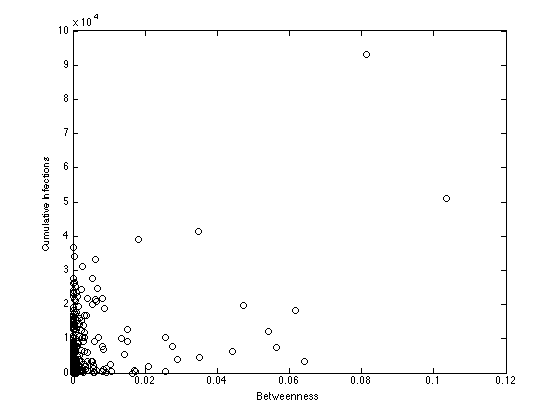
\includegraphics[width=7cm]{influ4}
\caption{sdlhfa}
\label{Betweenness}
\end{figure}

Figure \ref{Betweenness} shows, that high cumulative infection value implies high betweenness. But as we can also see in figure 3, it doesn't really imply the other direction.





